\subsection{Broadcasting}
\begin{frame}[fragile]
 Computing a 3D grid of distances $R_{ijk} = \sqrt(i^2 + j^2 + k^2)$
 \begin{block}{With temporary matrices}
   \begin{minted}{python}
In [44]: i, j, k = np.mgrid[-100:100, -100:100, -100:100]
In [45]: print(i.shape, j.shape, k.shape)
((200, 200, 200), (200, 200, 200), (200, 200, 200)

In [46]: R = np.sqrt(i**2 + j**2 + k**2)
In [47]: R.shape
Out[47]: (200, 200, 200)
\end{minted}
\end{block}
\end{frame}

\begin{frame}[fragile]
 Computing a 3D grid of distances $R_{ijk} = \sqrt(i^2 + j^2 + k^2)$
 \begin{block}{With temporary matrices}
   \begin{minted}{python}
# Construct the row vector that runs from -100 to +100
In [47]: i = np.arange(-100, 100).reshape(200, 1, 1)
#  Construct the column vector
In [48]: j = np.reshape(i, (1, 200, 1))
# Construct the depth vector
In [49]: k = np.reshape(i, (1, 1, 200))

In [50]: R = np.sqrt(i**2 + j**2 + ....: k**2)
In [51]: R.shape Out[49]: (200, 200, 200)
\end{minted}
 \end{block}
\end{frame}

\begin{frame}[fragile]
 Computing a 3D grid of distances $R_{ijk} = \sqrt(i^2 + j^2 + k^2)$
 \begin{center}
   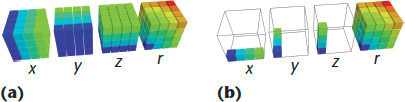
\includegraphics[scale=.5]{../figures/numpy/broadcasting.png}
 \end{center}
\end{frame}
